%
% fermat.tex -- Fermat-Prinzip, Brechungsgesetz als Minimalprinzip
%
% (c) 2021 Prof Dr Andreas Müller, OST Ostschweizer Fachhochschule
%
\bgroup
\begin{frame}[t]
\setlength{\abovedisplayskip}{5pt}
\setlength{\belowdisplayskip}{5pt}
\frametitle{Fermat-Prinzip}
\vspace{-20pt}
\begin{columns}[t,onlytextwidth]
\begin{column}{0.48\textwidth}
\begin{block}{Warum?\strut}
Welches physikalische Prinzip führt zum Brechungsgesetz?
\end{block}
\uncover<2->{
\begin{block}{Fermat-Prinzip\strut}
Licht wählt immer den schnellsten Weg
\end{block}
}
\uncover<4->{%
\begin{block}{Zeit im Medium $i$\strut}
\[
\only<4>{
t_i
=
\frac{
\sqrt{y_i^2+(x-x_i)^2}
}{
c/n_i
}}
\only<5>{t_i=
\frac{n_i}{c}
\sqrt{y_i^2+(x-x_i)^2}
}
\only<6->{
{\color<7->{red}t}
=
t_1+t_2
=
\frac{1}{c}\sum_{i=1}^n
n_i\sqrt{y_i^2+(x-x_i)^2}
}
\]
\end{block}}
\end{column}
\begin{column}{0.48\textwidth}
\begin{center}
\def\x{0.9}
\def\xone{-2}
\def\xtwo{2}
\def\yone{1.5}
\def\ytwo{-1.5}
\def\none{1}
\def\ntwo{1.5}
\def\s{1.5}
\def\o{5.8}
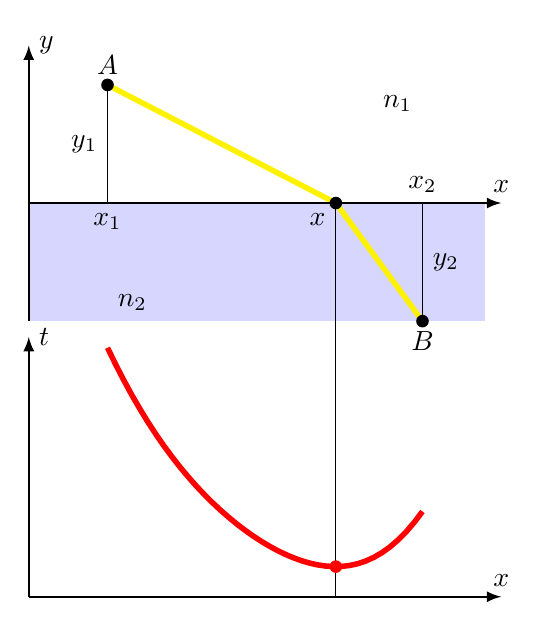
\begin{tikzpicture}[>=latex,thick]
\coordinate (A) at (\xone,\yone);
\coordinate (B) at (\xtwo,\ytwo);
\fill[color=blue!40,opacity=0.4] (-3,0) rectangle (2.8,-1.5);
%\uncover<3->{
	\node at (\xtwo,\yone) [below left] {$n_1$};
	\node at (\xone,\ytwo) [above right] {$n_2$};
%}
\draw[color=yellow,line width=2pt] (A) -- (\x,0) -- (B);
\draw[->] (-3,0) -- (3,0) coordinate[label={$x$}];
\draw[->] (-3,-1.5) -- (-3,2) coordinate[label={right:$y$}];
\uncover<3->{
	\draw[line width=0.3pt] (\xone,0) -- (A);
	\node at (\xone,0.75) [left] {$y_1$};
	\node at (\xone,0) [below] {$x_1$};
	\draw[line width=0.3pt] (2,0) -- (B);
	\node at (\xtwo,-0.75) [right] {$y_2$};
	\node at (\xtwo,0) [above] {$x_2$};
	\node at (\x,0) [below left] {$x$};
}
\fill (A) circle[radius=0.08];
\node at (A) [above] {$A$};
\fill (B) circle[radius=0.08];
\node at (B) [below] {$B$};
\fill (\x,0) circle[radius=0.08];
\uncover<7->{
	\draw[line width=0.3pt] (\x,0) -- (\x,-5);
	\fill[color=red] 
		({\x},{-5+\s*(\none*sqrt(\yone*\yone+(\x-\xone)*(\x-\xone))+\ntwo*sqrt(\ytwo*\ytwo+(\x-\xtwo)*(\x-\xtwo))-\o)})
		circle[radius=0.08];

	\begin{scope}[yshift=-5cm]
		\draw[color=red,line width=2pt] 
			plot[domain=\xone:\xtwo,samples=40]
				({\x},{\s*(\none*sqrt(\yone*\yone+(\x-\xone)*(\x-\xone))+\ntwo*sqrt(\ytwo*\ytwo+(\x-\xtwo)*(\x-\xtwo))-\o)});
		\draw[->] (-3,0) -- (-3,3.3) coordinate[label={right:$t$}];
		\draw[->] (-3,0) -- (3,0) coordinate[label={$x$}];
	\end{scope}
}
\end{tikzpicture}
\end{center}
\end{column}
\end{columns}
\end{frame}
\egroup
